\chapter{Prefaci}

\noindent
\textbf{Alan Kay}

President, \emph{Viewpoints Research Institute, Inc.} \&

Sr. Fellow, \emph{Hewlett-Packard Company}

\section*{El futur de la programació, vist des dels anys 60}

Vaig començar el doctorat (a la Universitat de Utah, dins el projecte ARPA) el novembre de 1966, i val a dir que és interessant mirar enrera al món de la programació tal com jo el veia aleshores.

L'extraordinària Jean Sammit (que va ser inventora de diversos llenguatges de programació i la seva primera historiadora, així com la primera dona presidenta de l'ACM) va comptar uns 3.000 llenguatges de programació utilitzats activament a finals dels anys 60. S'estava treballant molt en aquest camp, i part d'aquesta feina era molt important i molt interessant.

Algol 60, tal com Tony Hoare va assenyalar, ``va ser una enorme millora, especialment respecte als seus successors!''.  Tenia moltes virtuts, incloent més èmfasi en els contextos i els entorns dins la seva semàntica i una característica remarcable pel seu moment, la crida per nom (\emph{call by name}) que permetia als programadors una capacitat d'expressió similar a la dels mateixos dissenyadors del llenguatge. Per exemple, hom podia escriure accions que tinguessin el mateix significat i la mateixa execució que les instruccions de control pròpies del llenguatge:

\begin{verbatim}
for (i, 1, 10, print(a[i]))
\end{verbatim}

\noindent
on el primer i el quart paràmetres es marcarien com a \textsf{name} i així s'integrarien en una expressió que seria capaç de recordar correctament l'espai de noms jeràrquic al que pertanyen les seves variables, però que a més podia ser manipulat i executat des de dins el cos de l'acció \textsf{for}. Ni el LISP original va implementar correctament això al principi!

I hi havia una variant sintàctica poc coneguda en la sintaxi oficial d'Algol 60 que promovia una forma més llegible per a les accions definides per l'usuari. Això permetia que una coma en una crida a una acció pogués ser substituïda per la següent construcció:

\begin{verbatim}
): comentari (
\end{verbatim}

\noindent
la qual cosa hagués permès que la crida precedent fos escrita de la següent manera:

\begin{verbatim}
for (i): desde (1): fins (10): fer (print(a[i]))
\end{verbatim}

\noindent
Si féssiu això en una pantalla o en una IBM \emph{Executive typewriter} convertida en terminal (tal com podíeu fer amb JOSS) obtindríeu:

\vspace{5mm}
\noindent
\textsf{{\bfseries for} (i): {\bfseries desde} (1): {\bfseries fins} (10): {\bfseries fer} (print(a[i]))}
\vspace{5mm}

\noindent
que és ben bé com el llenguatge Algol de base, però amb una meta-extensió afegida pel programador en benefici d'altres programadors.

És possible que el conjunt d'idees i representacions més profundes al voltant dels llenguatges de programació succeís abans d'Algol, però van trigar força a ser enteses pels informàtics (i molts mai no les van entendre), en part per  una notació diferent i difícil de llegir (per gent de fora, si més no), i perquè moltes de les millors aportacions de LISP eren ``realment meta''. Una de les grans contribucions de LISP va ser el seu avaluador escrit en LISP mateix, en mitja pàgina de codi. Això va ser una mena d'\textsf{equacions de Maxwell} per a la programació, i va permetre pensar moltes coses que eren impensables amb els enfocaments habituals.


LISP mateix va ser utilitzat per ser el sistema en el que es va programar l'\emph{Advice Taker}, un agent interactiu amb sentit comú, que podia entendre els desitjos humans expressats en llenguatge natural i els transformava en processos informàtics que duien a terme aquells mateixos desitjos. A mitjans dels anys 60 es van crear alguns llenguatges intermedis interessants, com FLIP, i intents de reproduir part de les propietats de l'\emph{Advice Taker}, com PILOT.

Sketchpad potser va ser el més radical d'aquests sistemes desenvolupats inicialment, ja que va intentar proposar directament un marc raonablement interactiu per usuaris que volien utilitzar l'ordinador per fer allò pel que està millor preparat: tota mena de simulacions interactives. Les tres grans contribucions d'Sketchpad van ser:
\begin{itemize}
\item La primera aproximació utilitzable als gràfics interactius per ordinador.
\item Una veritable estructura d'objectes per a totes les seves entitats.
\item Una manera declarativa de programar en termes dels resultats finals desitjats, on el sistema podia utilitzar diversos mètodes automàtics de resolució de problemes per aconseguir els resultats buscats.
\end{itemize}

Això va ser impulsat tremendament per una ``aproximació tolerant'' a resoldre restriccions, on, en lloc de procurar trobar solucions logico simbòliques perfectes pels conjunts de restriccions, les restriccions s'intentaven resoldre amb toleràncies de tipus global. Aquesta manera de fer va permetre aproximar la solució de problemes importants que avui dia són difícils de resoldre o fins i tot intractables.

JOSS era tota una altra cosa: no feia ``pràcticament res'' (bàsicament càlcul numèric utilitzant nombres i taules), però el que feia ho feia perfectament; fins i tot ara podem considerar que tenia una de les millors interfícies d'usuari de la història.

\emph{A Programming Language} era el títol d'un llibre de Kenneth Iverson que va adoptar un enfoc fortament matemàtic a la programació, via funcions i meta-funcions expressades en una mena d'àlgebra. El llenguatge definit al llibre va rebre el nom d'``Iverson''. Un sistema real amb què es pogués programar un ordinador existia només com a rumor dins d'IBM en aquells temps, però sobre el paper es van escriure molts programes utilitzant aquestes idees. El millor d'Iverson era que realment sortia a compte si s'hi pensava en termes de transformacions i relacions matemàtiques, i no es considerava gaire el cost de les operacions. No preocupar-se pel cost era quasi impensable en aquells dies de rellotges d'1Mhz en ordinadors de la mida d'edificis i preus de millions de dòlars, per tant Iverson i LISP eren vehicles alliberadors a l'hora de pensar en el futur, un temps en el qual les màquines serien més petites i més ràpides.

Els dissenyadors de Simula volien modelitzar estructures dinàmiques grans i complexes i van adonar-se que els blocs d'Algol podien fer el fet si s'aconseguia alliberar-los de l'estricta estructura de control jeràrquica d'Algol. Quan van crear Simula I a mitjans dels anys 60 van ser capaços de veure que les seves idees eren força importants per al llenguatge i la seva programació, i quan van fer Simula 67 van poder reemplaçar molts tipus de dades que venien incorporats, com l'\textsf{string}, amb classes de Simula 67.

La idea d'extendre la sintaxi, la semàntica i la pragmàtica dels llenguatges de programació era tot un camp de recerca a mitjans i finals dels anys 60. Una de les raons d'això és que estava molt clar que la programació és una tasca on és difícil canviar d'escala, i que l'escalabilitat en moltes dimensions seria crítica per a la salut de la informàtica. On la complexitat és un problema central, l'arquitectura preval sobre els materials. La comprensió d'aquesta idea va fer que es comencés a veure que la programació és diferent de les matemàtiques, tot entenent-la com una nova forma d'enginyeria. Hi va haver propostes per a la formació d'una nova disciplina anomenada ``Enginyeria del Software'', i per a conferències, amb l'únic propòsit de treure l'aigua clara sobre el significat d'aquest nou nom (què fer quan no pots fer només matemàtiques).

L'\emph{Information Processing Techniques Office} (IPTO) de l'ARPA estava en plena activitat quan vaig començar el doctorat l'any 1966, i ja tenia en marxa uns quants projectes cap al somni col·lectiu de tenir computació interactiva per a tothom, connectats via una ``xarxa intergalàctica''. Intentar construir aquesta xarxa (amb importants requeriments d'escala) va generar part de les millors idees en sistemes informàtics de l'època, i va ser part important de les meves reflexions sobre el futur de la programació.

Els proveïdors de finançament d'ARPA van ser llestos i no van transformar la visió i el somni en objectius financers, en lloc d'això, van intentar trobar i finançar individus amb talent que tenien les seves pròpies idees sobre què significava el somni i com podia ser implementat. Això va donar lloc a uns 17 grups dins d'universitats i empreses, la majoria dels quals van proposar diferents dissenys i demostracions molt interessants. Així es va consituir una comunitat tant de discussió com de col·laboració que va fer a tothom que hi pertanyia més llest del que era abans d'afegir-s'hi.

Naturalment, donats els 3.000 llenguatges de Jean Sammit, hi ha molt que no he explicat, igual que molts dissenys interessants que s'han dut a terme des de 1967 fins al final de la dècada dels 70. Per triar només cinc desenvolupaments de particular importància per als lectors d'aquest llibre, jo em quedaria amb la meva pròpia concepció dels objectes i com se suposa que havien de ser útils als usuaris d'ordinadors personals; PLANNER, de Carl Hewitt, que era el sistema més cohesiu per practicar la ``programació com a raonament''; IMP, de Ned Iron, que representa potser el primer llenguatge útil completament extensible; i el \emph{Control Definition Language} de Dave Fisher, que va il·luminar les propietats d'extensibilitat en general i les de les estructures de control en particular.

Em vaig formar en matemàtiques, en biologia molecular (vaig pagar-me els estudis com a programador) i en art. Diverses circumstàncies van portar-me a haver d'entendre Sketchpad, Simula i la xarxa intergal·làctica proposada per ARPA en la meva primera setmana dins l'escola de doctorat, i la reacció que això em va provocar va ser cataclísmica. Eren similars en alguns aspectes i diferents en d'altres, però eren diverses espècies del mateix gènere, si hom prenia un punt de vista tant biològic com matemàtic. Biològicament, eren ``quasi cèl·lules'' demanant ser cèl·lules. Matemàticament, eren ``quasi àlgebres'' demanant ser àlgebres. Així, la meva fusió inicial d'aquestes metàfores amb la computació va donar lloc a la idea que es podia fer qualsevol cosa a partir d'entitats que hom podia considerar ordinadors virtuals amb la capacitat d'enviar missatges (els quals havien de ser també ordinadors virtuals). Els ordinadors virtuals actuarien com a cèl·lules i els protocols inventats podien ser força algebraics -el que avui dia anomenem (incorrectament) \emph{polimorfisme}. Això donaria lloc a una simplicitat i escalabilitat més gran a ``nivell dels materials'', i obriria la porta a progressos en simplicitat i escalabilitat al ``nivell de les expressions'', que és on viu el programador.

Alguns anys després vaig trobar PLANNER, de C. Hewitt, i em vaig adonar que aquella era la manera de fer programes més expressius i escalables (moltes de les idees de PLANNER van aparèixer després  en el llenguatge Prolog). Estava força clar que intentar enviar missatges orientats als objectius podia incrementar l'escalabilitat, en part perquè hi ha moltes més maneres d'intentar satisfer objectius que objectius (penseu a ordenar com a objectiu i en totes les maneres que hi ha d'ordenar), i aquesta separació podia proporcionar beneficis alhora mantenint els programes més expressius i menys barrejats amb altres problemes com l'optimització.

Mentrestant,  va aparèixer el llenguatge extensible IMP, amb algunes bones idees que en van fer un llenguatge pràctic, i no satisfet únicament amb les seves capacitats ``meta''.

I, en paral·lel amb la tesi en què jo estava treballant sobre ordinadors personals i sistemes orientats a objectes per a tota mena d'usuaris, Dave Fisher estava treballant en un conjunt complementari d'idees molt maques sobre com fer les estructures de control extensibles via la capacitat d'afegir nova semàntica dinàmicament a un meta-interpret de l'estil de LISP.

LOGO, el primer gran llenguatge de programació per a nens, era una combinació encertada de JOSS i LISP, feta per Papert, Feurzig, Bobrow i altres a BBN. Això va introduir la idea dels nens com a usuaris finals d'idees poderoses en computació, i va transformar la meva idea de la computació com a eina o vehicle en una idea de la computació com a \emph{mitjà} d'expressió amb un destí còsmic similar al de la impremta.

Aquest cinc sistemes i la invitació per ajudar a arrencar Xerox PARC van ser l'empenta per a Smalltalk, la qual cosa es deixa veure més en les seves primeres versions.

Mirant enrera, és sorprenent que:
\begin{itemize}
\item L'expressivitat dels llenguatges de programació actuals sigui tan baixa (a l'alçada del que hi havia cap el 1965) i que poquíssims programadors treballin al nivell que LISP o Smalltalk ja feien possible en els anys 70.
\item Smalltalk no ha canviat apreciablement des que va sortir la versió avui coneguda com Smalltalk-80, fins i tot considerant que conté el seu propi meta-sistema i que per tant és molt senzill de millorar.
\item La llei de Moore de 1965 ha resultat ser força correcte, i ara podem construir maquinari i programari molt grans, tot i que també molt fràgils, ja que no han estat considerats els conceptes escalables més enllà de la visió simple dels objectes (potser tenim ``cèl·lules'', però no conceptes equivalents als teixits, o com fer crèixer o construir organismes multi-cel·lulars).
\item Internet ha acabat sent l'expressió amb èxit d'una aproximació radical a l'arquitectura i a l'escalabilitat, tot i així, cap programari o sistema de programació ha estat preparat per a que els programadors puguin expressar sistemes similars a Internet.
\end{itemize}

Què ha passat amb el progrés en els darrers 25 anys? I per què Squeak és essencialment només un Smalltalk gratuït, si necessitem progressar desesperadament?

Al 1995 Internet era prou madura per intentar alguns experiments amb \emph{media} que feia temps que volíem fer. I el Java (i altres llenguatges) de l'època (i el d'ara) era força defectuós en aspectes com la flexibilitat, les capacitats ``meta''  i la portabilitat com per ser-nos un vehicle útil. Ja havíem fet Smalltalk abans, i havíem escrit un llibre sobre com construir-ne un sistema complet, era per tant raonable prendre's un any per fer un Smalltalk gratuït i controlable i distribuir-lo per Internet (de fet, ens va portar uns nou mesos). La idea era que Squeak no hauria de ser un vehicle sinó una fàbrica per a un llenguatge del segle XXI que fos molt millor.

Malgrat tot, els sistemes de programació amb què els programadors treballen sovint tenen vida pròpia, i gran part del moviment \emph{open source} al voltant d'Squeak va mostrar-se més interessat en un Smalltalk gratuït amb un sistema multimèdia portable. Crec que és raonable afirmar que la majoria de la comunitat Squeak està dedicada a fer aquest Smalltalk més útil i accessible, i no pas a fer alguna altra opció que deixi Smalltalk obsolet (un destí que m'encantaria veure realitzat).

Per això, m'agradaria encoratjar els lectors d'aquest nou i excel·lent llibre a no pensar Smalltalk com un conjunt de característiques imposades pels venedors a les que ens hem de resignar, sinó com un  sistema que és capaç de ser ampliat en totes les seves dimensions i que recompensarà tots aquells que inventin noves i millors maneres de programar. Al PARC nosaltres canviàvem Smalltalk cada poques setmanes, i d'una manera significativa cada dos anys. Encara que amb prou feines ha canviat des d'aleshores, si us plau proveu de canviar-lo, i poseu aquestes modificacions a Internet perquè tots en puguem aprendre i gaudir!

\chapter{Sobre l'autor}

\noindent
\textbf{STÉPHANE DUCASSE} va obtenir el seu doctorat a la Universitat de Nice-Sophia Antipolis i la seva habilitació a la Universitat de París 6. Va rebre el premi SNF 2002 \emph{Professeur Boursier}. Actualment és professor a la Universitat de Berna i a la Universitat de Savoie\footnote{\emph{Nota del Traductor}: Actualment (gener 2008) és director de recerca a l'INRIA (Lille, França)}.

\vspace{5mm}
\noindent
Les arees d'interès de Stéphane són el disseny de sistemes reflexius, el disseny de llenguatges orientats a objectes, els components de programari, el disseny i la implementació d'aplicacions, la re-enginyeria d'aplicacions orientades a objectes i l'ensenyament. És el desenvolupador principal del \emph{Moose Reengineering Environment}. Adora programar en Smalltalk i és president de l'ESUG (\emph{European Smalltalk Users Group}).

\vspace{5mm}
\noindent
Stéphane ha escrit diversos llibres en francès i anglès: \emph{La programmation: une approche fonctionnelle et recursive en Scheme} (Eyrolles, 1996), \emph{Squeak} (Eyrolles, 2001), i \emph{Object-Oriented Reengineering Patterns} (MKP, 2001).

\vspace{5mm}
\noindent
Si vols descobrir perquè Stéphane es diverteix amb Squeak i participa activament en el seu desenvolupament, visita
\textsf{http://www.squeak.org}.

\vspace{5mm}
\noindent
Visita \textsf{http://smallwiki.unibe.ch/botsinc} pel lloc web d'aquest llibre\footnote{\emph{Nota del Traductor}: En anglès}.


\chapter{Agraïments}

\noindent
És un plaer donar-vos les gràcies a tots aquells de vosaltres que heu llegit parts i esborranys d'aquest llibre i m'heu donat \emph{feedback}. No és senzill llegir un treball inacabat,  i us agraeixo que hagueu fet l'esforç. No intentaré llistar els vostres noms aquí, ja que segurament oblidaria algú. Tot i així, hauria de mencionar l'Orla Greevy, l'Ian Prince i en Daniel Knierim, que van llegir el manuscrit sencer. Gràcies pel vostre \emph{feedback} i recolzament. També m'agradaria mencionar en particular el Daniel Villain, que va llegir un esborrany de la versió francesa.

\vspace{5mm}
\noindent
Voldria agrair a la comunitat Squeak per l'ajut proporcionat mentre desenvolupava els entorns que utilitzo en aquest llibre, i per desenvolupar aquest entorn tan magnífic que és Squeak, principalment. En particular, vull agrair al Nathanel Schärli i al Ned Konz el seu ajut. Agraïments especials a tots aquells desenvolupadors que han ajudat Smalltalk a deixar de ser un somni i esdevenir una realitat. També m'agradaria donar les gràcies a tots els ``Smalltalkers'' que han fet d'aquest llenguatge i aquesta comunitat quelcom tan emocionant. Que continueu fent realitat els vostres somnis.

\vspace{5mm}
\noindent
Escriure aquest llibre ha estat un procés llarg i complicat, ja que ensenyar novells és difícil. És més, no sóc una persona amb qui sigui fàcil conviure, i com a investigador, m'emocionen massa temes. Vull agrair particularment Didier Besset les discussions molt fructíferes al començament d'aquest projecte.

\vspace{5mm}
\noindent
També voldria donar les gràcies a la meva esposa, la Florence, i els meus fills el Quentin i el Thibaut, dos noiets a qui encantava córrer sorollosament al voltant de la taula mentre intentava concentrar-me en la meva feina. Gràcies per acceptar un marit i un pare que no era sempre present, entusiasta ni accessible. Aviat estarem programant junts.

\chapter{Nota del traductor}

\noindent
Aquest llibre que teniu entre mans és la traducció al català del llibre del professor Stéphane Ducasse:

\vspace*{3mm}

\noindent
\begin{itemize}
\item[] \textsf{Squeak: Learn Programming with Robots} \\ 
Stéphane Ducasse, APress 2005\\
ISBN:1-59059-491-6
\end{itemize}

\vspace*{3mm}

\noindent
El programari \textsf{BotsInc} que acompanya al llibre en anglès el teniu a 

\noindent
\textsf{http://smallwiki.unibe.ch/botsinc/download/}

\vspace*{3mm}

\noindent
Teniu una traducció parcial al català d'aquest programari a \textsf{http://citilab.eu}, que és la que he utilitzat en aquesta traducció del llibre. S'han traduït: Les classes associades a l'entorn \textsf{BotsInc} que són accessibles per a l'usuari, els noms dels colors (constructors de la classe \textsf{Color}), l'entorn (menús, halos, botons, etc), el mètode
\textsf{negated}  (classe \textsf{Number}, traduït com \textsf{negat}), i les següents estructures de control d'Smalltalk:
\textsf{timesRepeat:}  (classe \textsf{Integer}, traduït com \textsf{vegadesRepetir:}),
 \textsf{whileTrue}  (classe \textsf{BlockContext}, traduït com \textsf{mentreCert}),
 \textsf{whileTrue:}  (classe \textsf{BlockContext}, traduït com \textsf{mentreCert:}),
 \textsf{whileFalse}  (classe \textsf{BlockContext}, traduït com \textsf{mentreFals}),
 \textsf{whileFalse:}  (classe \textsf{BlockContext}, traduït com \textsf{mentreFals:}),
 \textsf{repeat}  (classe \textsf{BlockContext}, traduït com \textsf{repetir}),
 \textsf{ifTrue:}  (classes \textsf{True} i \textsf{False}, traduït com \textsf{siCert:}),
 \textsf{ifTrue:ifFalse:}  (classes \textsf{True} i \textsf{False}, traduït com \textsf{siCert:siFals:}),
 \textsf{ifFalse:}  (classes \textsf{True} i \textsf{False}, traduït com \textsf{siFals:}) i
 \textsf{ifFalse:ifTrue:}  (classes \textsf{True} i \textsf{False}, traduït com \textsf{siFals:siCert:}).

\noindent
Amb això ja podeu practicar, en català, la major part del contingut del llibre.

\vspace*{3mm}

\noindent
Ara bé, l'entorn \textsf{BotsInc} està implementat en Smalltalk dins de l'entorn Squeak (que és una implementació del llenguatge de programació Smalltalk). Per tant, el llibre fa servir moltes eines que són pròpies de l'entorn Squeak general i no estan especialment vinculades a \textsf{BotsInc}. Aquestes eines d'Squeak utilitzades en el llibre no han estat traduïdes. En concret, les eines són el depurador (\emph{debugger}), \emph{Paint} (per fer dibuixos) i el \emph{Transcript}. A més, ocasionalment s'utilitzen classes que pertanyen a Squeak (i no específicament a \textsf{BotsInc}) que tampoc han estat traduïdes: \textsf{World}, \textsf{Character}, \textsf{Magnitude}, \textsf{PopUpMenu}, \textsf{FillInTheBlank}, \textsf{String}, \textsf{Time}, \textsf{Date}, \textsf{Rectangle}, \textsf{Point} i \textsf{UndefinedObject}.

\vspace*{3mm}

\noindent
\textbf{\large Agraïments:}
Voldria agrair el suport que he tingut per fer aquesta traducció per part de:
\begin{itemize}
\item Stéphane Ducasse, per haver escrit un llibre tan adequat i pels seus esforços en fer accessible lliurement tant l'original com la traducció.
\item Citilab: Va ser un projecte que vaig començar amb ells que va motivar aquesta traducció. M'agradaria mencionar especialment en Ramón Sangüesa, per enredar-me, i en Joan Güell i en Josep Garcia, per seguir-me la veta en això de l'Smalltalk.
\item Softcatalà i el TERMCAT, per la seva valuosa tasca, que entre d'altres coses m'ha estalviat la feina d'introduir neologismes.
\item Pau Fernández, per fer-me descobrir l'Inkscape i per disculpar-me el temps que no li he dedicat com a director de tesi.
\item Lali Forcades, per fer que aquest llibre sembli escrit per algú que sap escriure en català.
\item La meva familia, per tolerar el temps robat.
\item Finalment, els estudiants que han volgut venir al curs inspirat per aquest llibre, per deixar-me experimentar i perllongar la seva paciència més enllà del que molts haguessin considerat raonable.
\end{itemize}

\vspace*{3mm}

\noindent
Voldria dedicar aquesta traducció a la Montse, la Marta i el Jaume. 
\vspace*{5mm}

\noindent
\begin{flushleft}
\textbf{Jordi Delgado}\\
\textsf{Citilab}, i Dept. Llenguatges i Sistemes Informàtics (UPC)\\
\textsf{jdelgado@lsi.upc.edu}\\
\end{flushleft}

\chapter{Pròleg}

\begin{quote}
\begin{flushright}
\emph{El coneixement és només una part de la comprensió.\\ 
L'autèntica comprensió ve de l'experiència}.\\
S. Papert
\end{flushright}
\end{quote}



\section*{Objectius i públic lector}

L'objectiu d'aquest llibre és explicar conceptes elementals de programació
(com l'abstracció, la composició, les repeticions o els condicionals) a novells 
de totes les edats. Crec que aprendre experimentant i resolent problemes és
fonamental en l'adquisició de coneixements. Per tant, introduiré conceptes
de programació a través de problemes senzills com ara dibuixar rectangles d'or
o simular el comportament animal.

El meu objectiu final és ensenyar-vos programació orientada a objectes, ja que
aquest paradigma particular proporciona una metàfora excel·lent per ensenyar a
programar. Tot i així, la programació orientada a objectes requereix algunes
nocions addicionals de programació i abstracció. Per tant, he escrit 
aquest llibre per introduir aquests conceptes de programació elementals en
un entorn de programació també elemental, amb la idea que sigui
el primer volum d'una sèrie de dos. Malgrat això, aquest llibre és completament 
autosuficient i no requereix que es llegeixi el segon volum. El segon llibre
introdueix un altre petit entorn de programació. Posa èmfasi en temes de nivell
intermedi com ara trobar un camí en un laberint o dibuixar fractals. També pot 
jugar el paper de llibre d'ampliació per a lectors que volen saber-ne més o que
volen adaptar l'entorn d'aquest llibre a les seves
necessitats. Finalment, s'introdueix la programació orientada a objectes.

El lector ideal que tinc al cap és un individu que vol divertir-se programant.
Aquest individu pot ser jove o adult, mestre d'escola o algú que ensenya als 
nens a programar. No cal que sigui hàbil programant en
cap altre llenguatge.

El material d'aquest llibre ha estat desenvolupat originalment per a la meva dona,
que és professora de física i matemàtiques en una escola francesa amb estudiants
d'entre onze i quinze anys. A finals de 1998, la meva dona es va fer càrrec 
d'ensenyar informàtica i es va quedar sorpresa per la manca de material adequat.
Va començar ensenyant HTML, Word i altres temes però no li van resultar
prou satisfactoris, ja que cap d'aquests ensenyaments no promou una 
actitud \textit{científica} cap a la informàtica. El seu objectiu era ensenyar 
informàtica com un procés de resolució de problemes.

Com a informàtic, jo era conscient de la feina que s'ha fet amb el llenguatge
de programació Logo, i em va agradar la idea de l'experimentació com a base de 
l'aprenentatge. També era conscient que el llenguatge de programació Smalltalk
ha estat influenciat per les idees de Seymour Papert per al llenguatge 
Logo, i que darrera del seu origen hi va haver força recerca en la manera d'ensenyar
a nens a programar. És més, Smaltalk té una sintaxi força senzilla que imita el
llenguatge natural. Més o menys per aquelles dates, l'entorn de programació 
Squeak havia arribat a un estat madur i van començar a aparèixer llibres sobre Squeak, cap a finals de 1999. Aquests, però, estaven destinats a programadors
amb experiència, de manera que m'hi vaig posar i vaig escriure aquest llibre que
teniu entre mans.

Els entorns que utilitzo en aquest llibre i el que l'acompanya són completament
funcionals. Els he anat millorant a partir de les respostes que he
rebut de professors i mestres. Ha estat una pauta en la meva feina 
modificar el mínim possible l'entorn Squeak, ja que el meu objectiu
és que els lectors d'aquest llibre ampliïn les idees aquí presents i ells
mateixos en desenvolupin de noves.

\section*{Estructura orientada a objectes i vocabulari}

Els capítols d'aquest llibre són relativament breus, de manera que cada 
capítol es pot convertir en sessions de laboratori d'una o dues hores.
No defensaré la idea d'introduir el material directament als nens per a l'auto-aprenentatge,
però cada capítol conté de fet tot el material que cal si es vol fer d'aquesta
manera.

Encara que la programació orientada a objectes no es desenvolupa en aquest 
llibre, utilitzo el seu vocabulari. És a dir, crearem objectes a partir de
classes i els enviarem missatges. El comportament dels objectes ve definit per
mètodes. He triat de fer-ho així ja que la metàfora que em proporciona la 
programació orientada a objectes és força natural, i els nens i nenes tenen una
comprensió intuïtiva dels objectes i del seu comportament.

Aquells que han utilitzat Logo es poden preguntar per quina raó els nostres
robots no disposen de l'operació ``llapis amunt'' i ``llapis avall'', enlloc
de ``ves'' i ``salta'', on la primera fa que un robot es mogui deixant una
traça i la darrera mou un robot sense deixar cap marca. Crec que el paradigma
que ens proporciona ``ves'' i ``salta'' s'adequa millor a les idees de la 
programació orientada a objectes i encapsulament de dades que el tradicional
disseny basat en ``llapis amunt'' i ``llapis avall''. Una anàlisi excel·lent 
d'aquestes dues perspectives va ser realitzada per Didier Besset, que va 
col·laborar amb mi al principi d'aquest projecte.

\section*{Organització}

El llibre està dividit en cinc parts, tal com està descrit més avall.

\paragraph{Començar.}  La primera part ens ensenya a engegar l'entorn Squeak. Explica
el procés d'instal·lació i d'arrencada d'Squeak, i després introdueix alguns 
robots amb el seu comportament. Es presenta un primer programa senzill per 
dibuixar algunes línies.

%% Aqui va la figura del quadrat que va girant
\vspace{5mm}
\includegraphics[height=20mm ,width=90mm ]{Imatges/Preface1.jpg}

\paragraph{Conceptes elementals de programació.} La segona part introdueix els 
primers conceptes de programació, com les repeticions i les variables. Mostra també com 
es resolen els missatges enviats a robots.

%% Aqui va la figura de l'espiral quadrada.
\vspace{5mm}
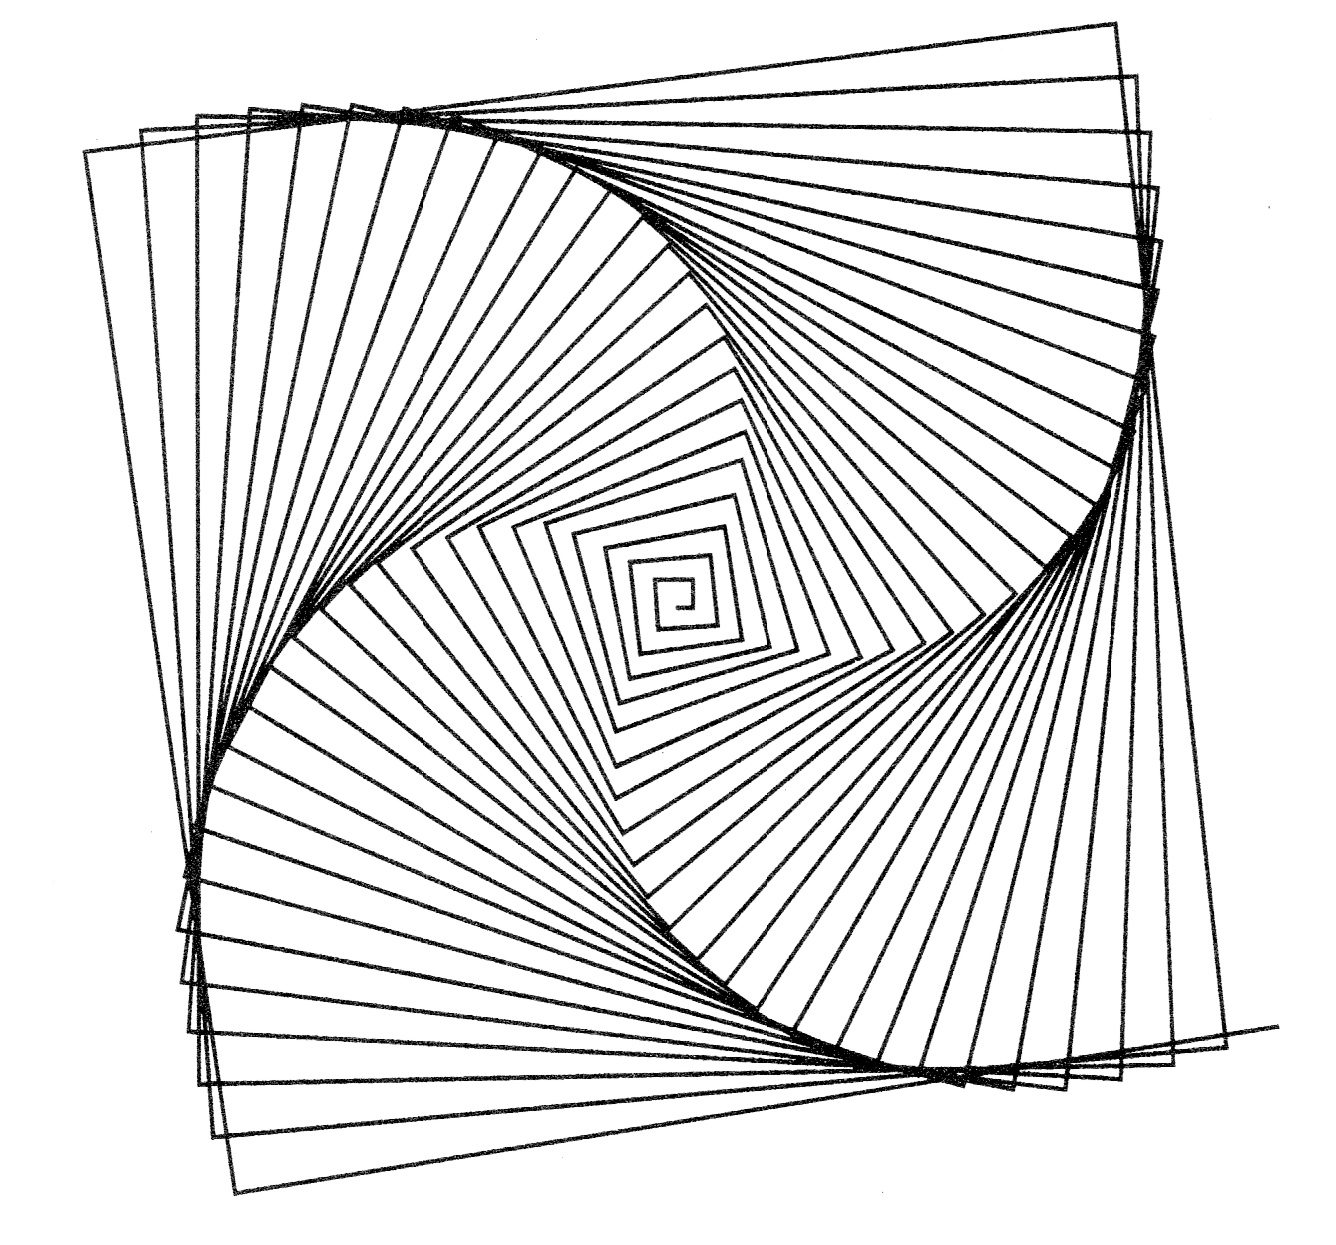
\includegraphics[height=40mm ,width=40mm ]{Imatges/Preface2.jpg}

\paragraph{Posar en joc l'abstracció.} La tercera part introdueix la necessitat de l'abstracció, és a dir, de mètodes
o procediments que poden ser reutilitzats per programes diferents. El concepte 
més difícil que s'introdueix és la idea de composar nous mètodes a partir de mètodes
ja existents per resoldre problemes més complexos. Proposaré diversos 
experiments no trivials, com ara dibuixar rectangles d'or. També introduirem
tècniques i eines per depurar (\textit{debug}) programes.

%% Aqui va la figura dels rectangles d'or
\vspace{5mm}
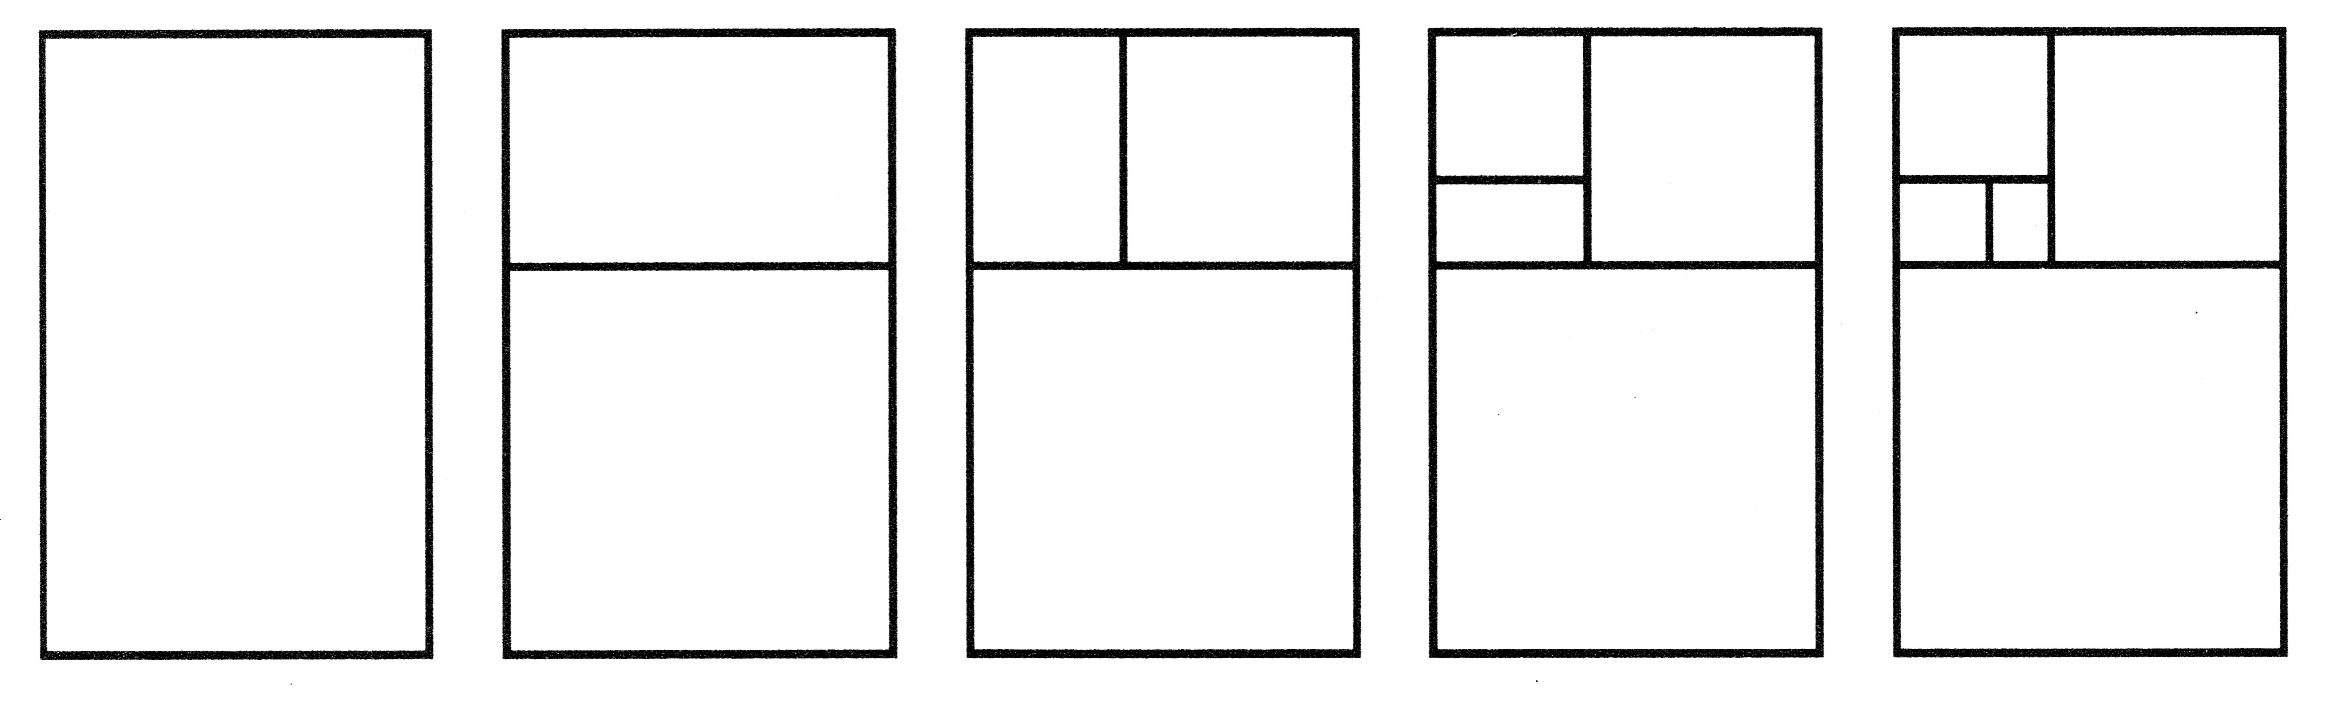
\includegraphics[height=30mm ,width=100mm ]{Imatges/Preface3.jpg}

\paragraph{Condicionals.} La quarta part introdueix les nocions de condicional, bucle condicional i 
expressió booleana, totes fonamentals per a la programació. Aquesta part 
explica també el concepte de referència en un espai bidimensional i altres
tipus de comportaments robòtics. Finalment, es presenten maneres d'utillitzar
els robots per simular el comportament d'animals simples.

%% Aqui va la figura dels comportaments d'animals
\vspace{5mm}
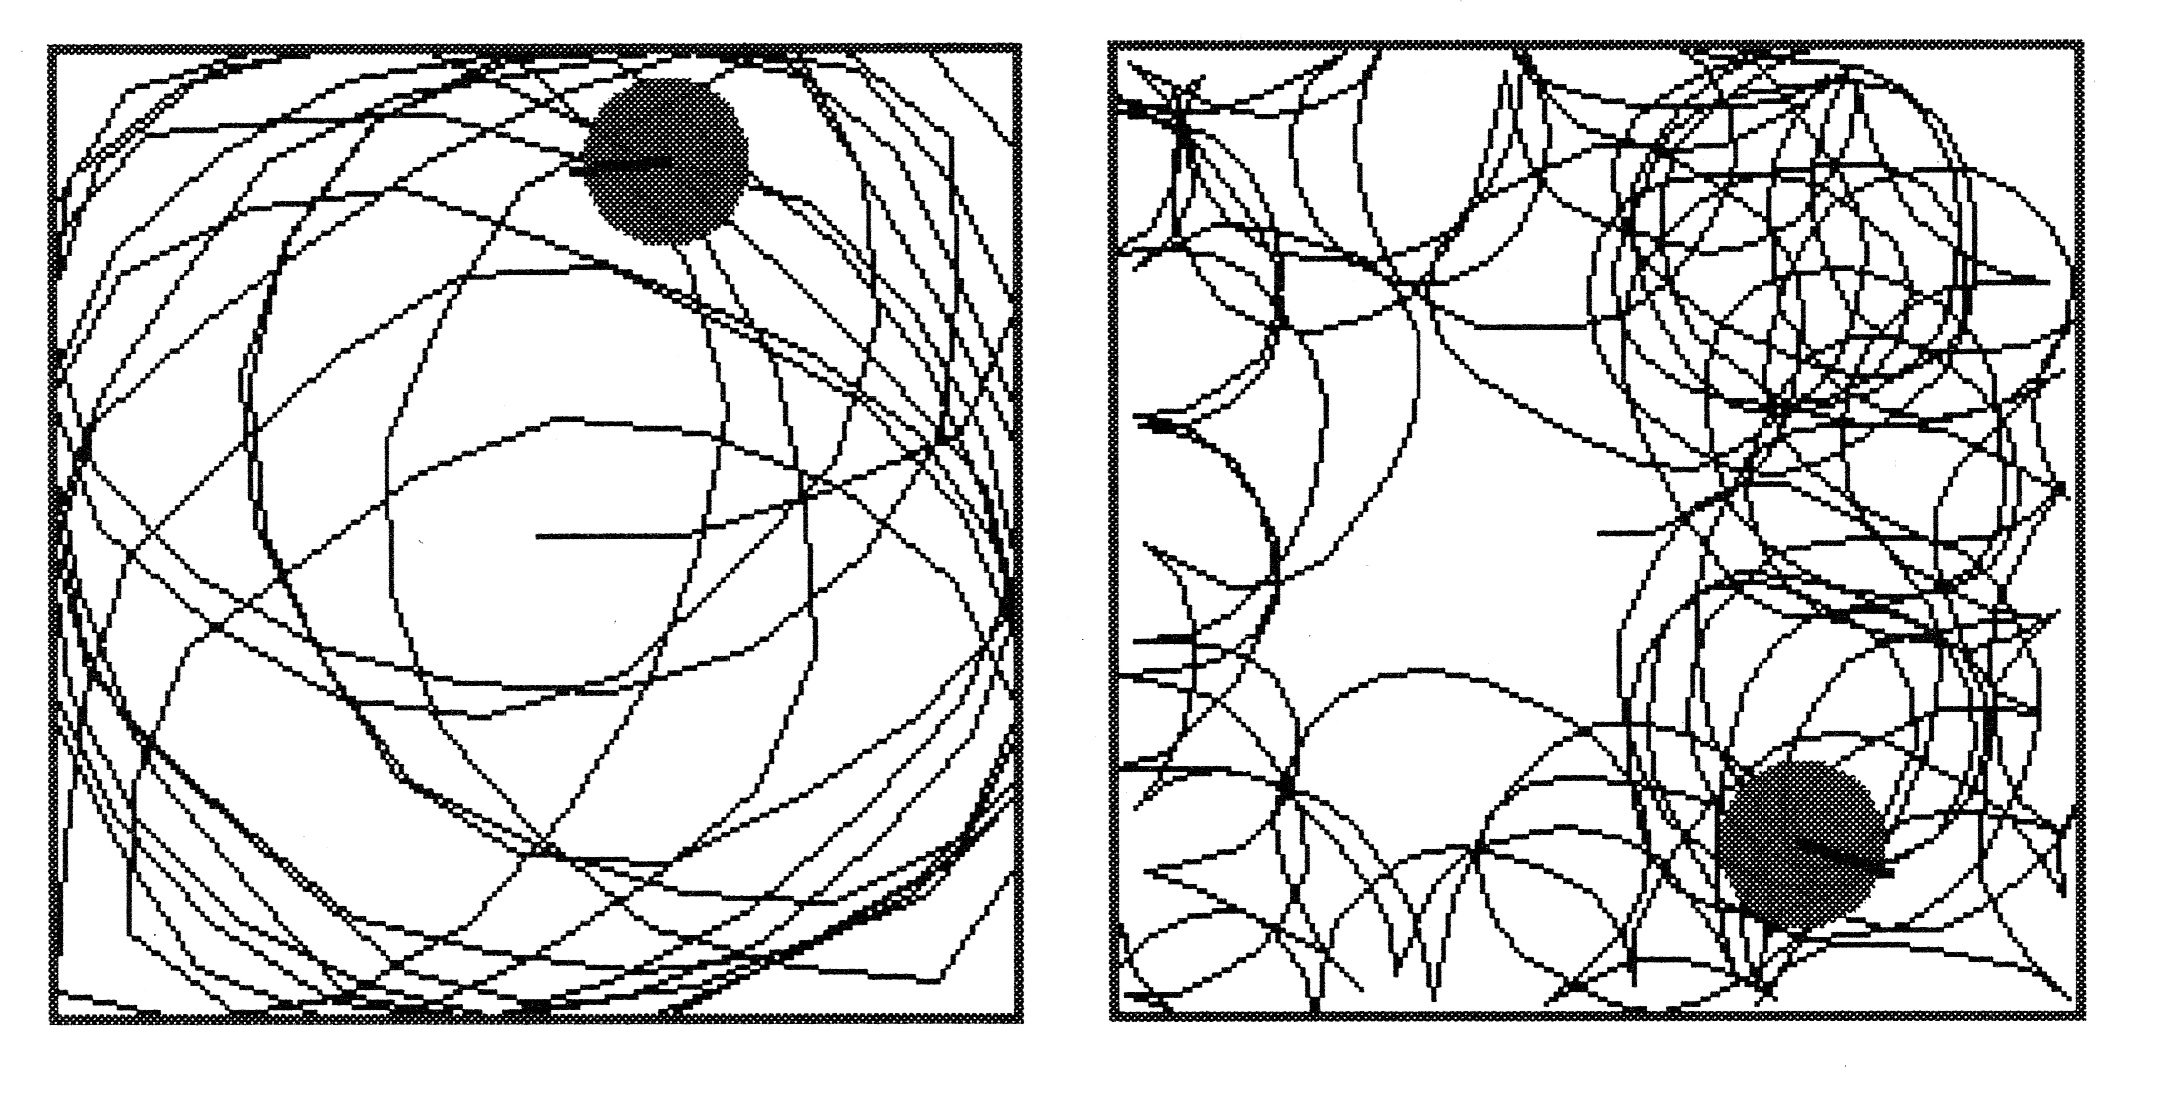
\includegraphics[height=45mm ,width=90mm ]{Imatges/Preface4.jpg}

\paragraph{Altres Mons Squeak.}
La cinquena part presenta dos entorns de programació força entretinguts que estan
disponibles en Squeak: el sistema d'\textit{scripting} gràfic \textsf{eToy} i l'entorn
\textsf{3D Alice}.

\section*{Per quina raó Squeak i Smalltalk?}

Podeu preguntar-vos perquè, d'entre el gran nombre de llenguatges de 
programació existents avui dia, he triat Smalltalk. Els he triat per les seguents raons:

\begin{itemize}
\item Smalltalk és un llenguatge molt potent. Podeu construir sistemes molt
complexos en un llenguatge que és simple i uniforme.
\item Smalltalk va ser dissenyat com un llenguatge per a l'ensenyament. Va inspirar-se
en Logo i en Lisp, i va influenciar fortament
llenguatges com Java o C\#. Tot i així, aquests llenguatges són massa complexos 
per a una primera aproximació a la programació. A més, han perdut la bellesa de
la simplicitat d'Smalltalk. 
\item Smalltalk és un llenguatge tipat dinàmicament i això torna irrellevants una
sèrie de qüestions relacionades amb tipus i coerció de tipus que són difícils
d'explicar i de poc interès pels neòfits.
\item Amb Smalltalk només cal aprendre conceptes clau, essencials, que es poden
trobar en tots els llenguatges de programació. Així, puc 
concentrar-me a explicar els conceptes importants sense haver de tractar altres
aspectes més difícils i poc atractius dels llenguatges més complexos.
\item Squeak és un potent entorn multimèdia, de manera que després de llegir 
aquests llibres hom podrà construir programes en un entorn 
realment ric.
\item Squeak està disponible gratuïtament i es pot executar en totes les 
plataformes principals. I hauria de ser fàcilment portable a altres
plataformes del futur.
\item Squeak és popular. Per exemple, a 
Espanya\footnote{\emph{Nota del traductor}: Ducasse es refereix a la 
utilització que es fa d'Squeak a Extremadura. \\ Veure \textsf{http://squeak.educarex.es/squeakpolis}} 
s'utilitza a les escoles, on s'executa en uns 80.000 ordinadors.
\end{itemize}

